Encuentra el valor de $x$ en el siguiente triángulo isóceles:

% \begin{minipage}[t][][t]{0.3\textwidth}
\begin{figure}[H]
    \centering
    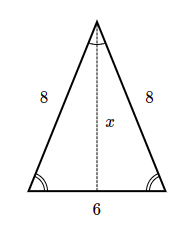
\includegraphics[width=0.2\linewidth]{../images/pitagoras0.png}
    \caption{}
    \label{fig:pitagoras0}
\end{figure}
% \end{minipage}\hfill
% \begin{minipage}[t][][t]{0.68\textwidth}
\begin{solutionbox}{15cm}
    \begin{minipage}{0.3\textwidth}
        \begin{figure}[H]
            \centering
            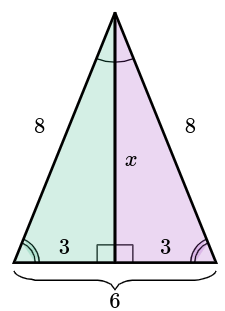
\includegraphics[width=0.6\linewidth]{../images/pitagoras0a.png}
            \caption{}
            \label{fig:pitagoras0a}
        \end{figure}
        \begin{figure}[H]
            \centering
            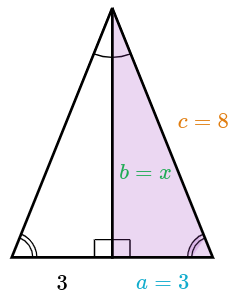
\includegraphics[width=0.6\linewidth]{../images/pitagoras0b.png}
            \caption{}
            \label{fig:pitagoras0b}
        \end{figure}
    \end{minipage}\hfill
    \begin{minipage}{0.65\textwidth}
        El triángulo isóceles está formado por 2 triángulos congruentes (ver Figura \ref{fig:pitagoras0a}).
        La base de cada triángulo rectángulo es la mitad de la base del triángulo isóceles.
        Cuando se trata de un triángulo rectángulo podemos utilizar el teorema de Pitágoras para encontrar un lado faltante.
        La ecuación del teorema de Pitágoras es:
        \[{\color{orange}c}^2={\color{cyan}a}^2+{\color{LimeGreen}b}^2\]
        donde $a$ y $b$ son las longitudes de los catetos, y $c$ es la longitud de la hipotenusa.
        Etiquetemos la Figura del problema con $a$, $b$ y $c$ (ver Figura \ref{fig:pitagoras0b}).
        Observa que $a$ y $b$ pueden intercambiarse, pues son catetos.
        \begin{align*}
            {\color{cyan}a}^2+{\color{LimeGreen}b}^2  ={\color{orange}c}^2 & \text{\quad El teorema de Pitágoras}                          \\
            {\color{cyan}3}^2+{\color{LimeGreen}x}^2  ={\color{orange}8}^2 & \text{\quad Sustituye las longitudes}                         \\
            9+x^2  =64                                                     & \text{\quad Evalua los cuadrados conocidos}                   \\
            x^2=64-9                                                       & \text{\quad Despejando } x                                    \\
            x^2=55                                                         & \text{\quad Restando}                                         \\
            x=\sqrt{55}                                                    & \text{\quad Calculando la raíz en ambos lados de la ecuación} \\
        \end{align*}
    \end{minipage}
\end{solutionbox}
% \end{minipage}
